\documentclass{standalone}
\usepackage{tikz}

\begin{document}

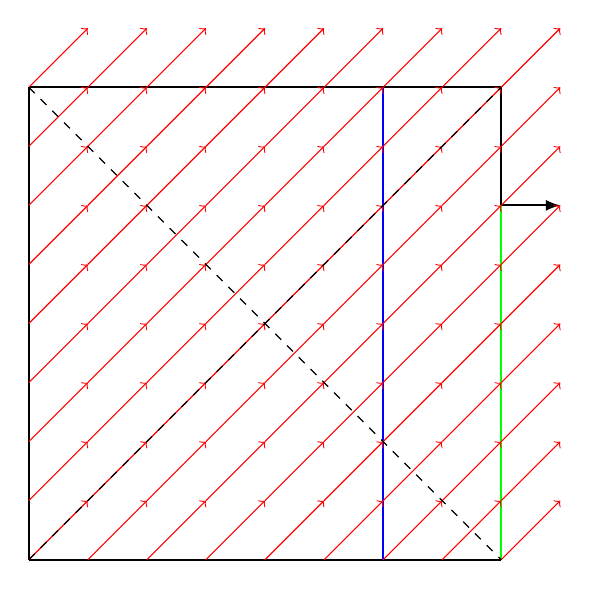
\begin{tikzpicture}[scale=1.5]

% Draw the main lines of the structure
\draw[thick] (0,0) -- (4,0);
\draw[thick] (0,0) -- (0,4);
\draw[thick] (4,0) -- (4,4);
\draw[thick] (0,4) -- (4,4);

% Draw the blue line
\draw[thick,blue] (3,0) -- (3,4);

% Draw the green line
\draw[thick,green] (4,0) -- (4,3);

% Draw the black arrow at the end of the green line
\draw[thick,black,-latex] (4,3) -- (4.5,3);

% Draw the red arrows
\foreach \x in {0,0.5,...,4}{
    \foreach \y in {0,0.5,...,4}{
        \draw[red,->] (\x,\y) -- ++(0.5,0.5);
    }
}

% Draw the dashed lines
\draw[dashed] (0,0) -- (4,4);
\draw[dashed] (0,4) -- (4,0);

\end{tikzpicture}

\end{document}